\chapter{Results and Validation}
\label{chapter:results_and_validation}

\section{Geographic Delimitation of the Simulation Domain}

Before analyzing the hydraulic outputs, it is necessary to define the spatial boundaries of the simulation grid. The 
computational domain developed for this study focuses strictly on the eastern coastal watershed within the Valencian 
Community (Spain), which sustained the most severe urban damage during the flash flood event of October 29, 2024.

To maintain an optimal balance between grid resolution ($5\text{ m} \times 5\text{ m}$ cells) and computational feasibility, 
other heavily affected regions have been explicitly excluded from this simulation. These include upstream high-altitude 
areas of the catchment (such as Utiel, in the interior of the Valencia province) as well as adjacent affected river basins 
located in the neighboring region of Castilla-La Mancha (e.g., Letur or Mira). The bounding box of the active simulation 
area covers a total surface of 1311 $\text{km}^2$, enclosing the critical urban corridors of the ground-zero zone.

\begin{figure}[htbp]
    \centering
    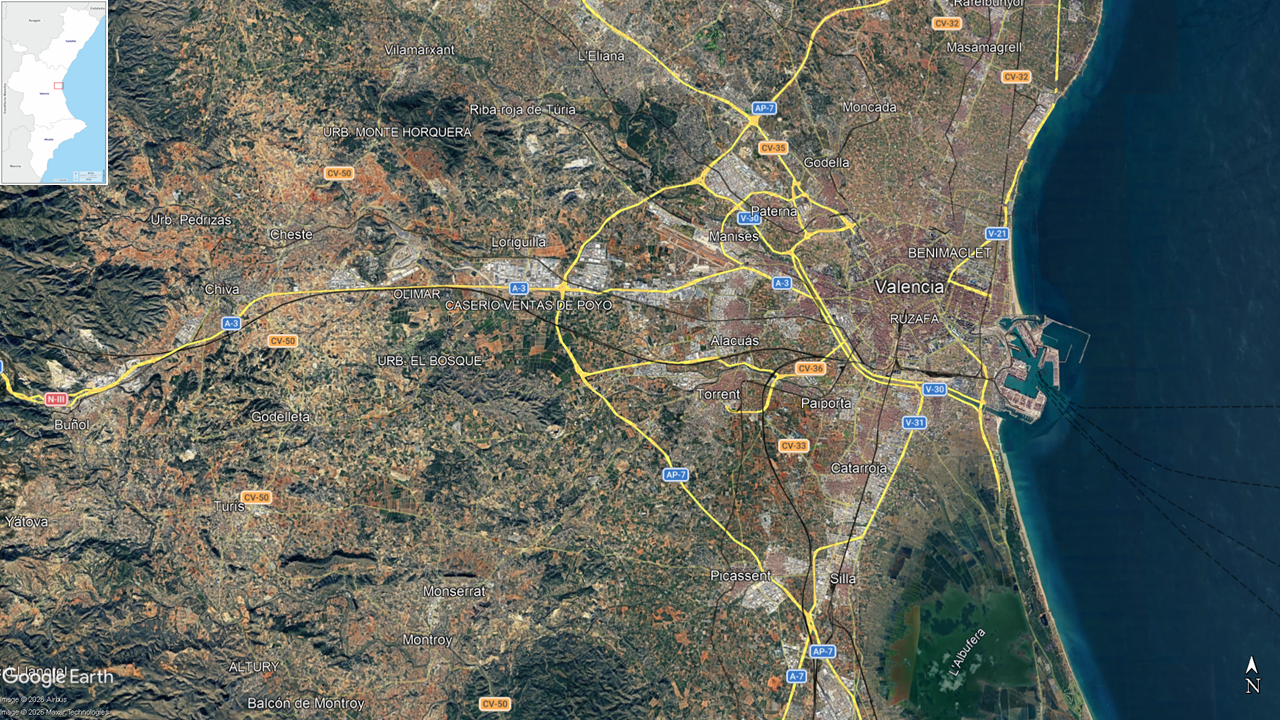
\includegraphics[width=0.9\textwidth]{images/results/topographic_overview.png}
    \caption{Topographic overview of the active simulation domain overlaid on a Google Earth satellite composite.}
    \label{fig:topographic_overview}
\end{figure}


\section{Hydraulic Scale and Color Representation}

To ensure quantitative readability across all bi-dimensional and tri-dimensional visual outputs, a standardized discrete 
color scale consisting of 15 intervals was defined. This chromatic framework is conceptually grounded in the classic 6-level 
flood hazard classification established by the Australian Emergency Management Institute and utilized by 
\cite{Smith2016} for estimating flood fatalities and identifying populations at risk based on vulnerability 
curves.

While the reference framework relies on six broader categories—utilizing critical thresholds such as $H5$ to define severe 
structural and life-safety risks (see Figure \ref{fig:original_hazard} for the original reference curves)—the scale proposed 
in this work expands these thresholds into 15 high-resolution intervals. This sub-discretization does not contradict the 
underlying physics of the original curves; rather, it introduces a tighter granularity specifically tailored to capture the 
full socio-environmental spectrum of this specific event. It filters out negligible hydraulic noise below 0.20 m and transitions 
smoothly from bright yellows to deep reds, magentas, and dark purples, allowing the visual outputs to clearly differentiate 
standard urban street flooding from the ultra-catastrophic submersion levels (exceeding 12.0 m) observed in the study area.

\begin{figure}[h!]
\centering
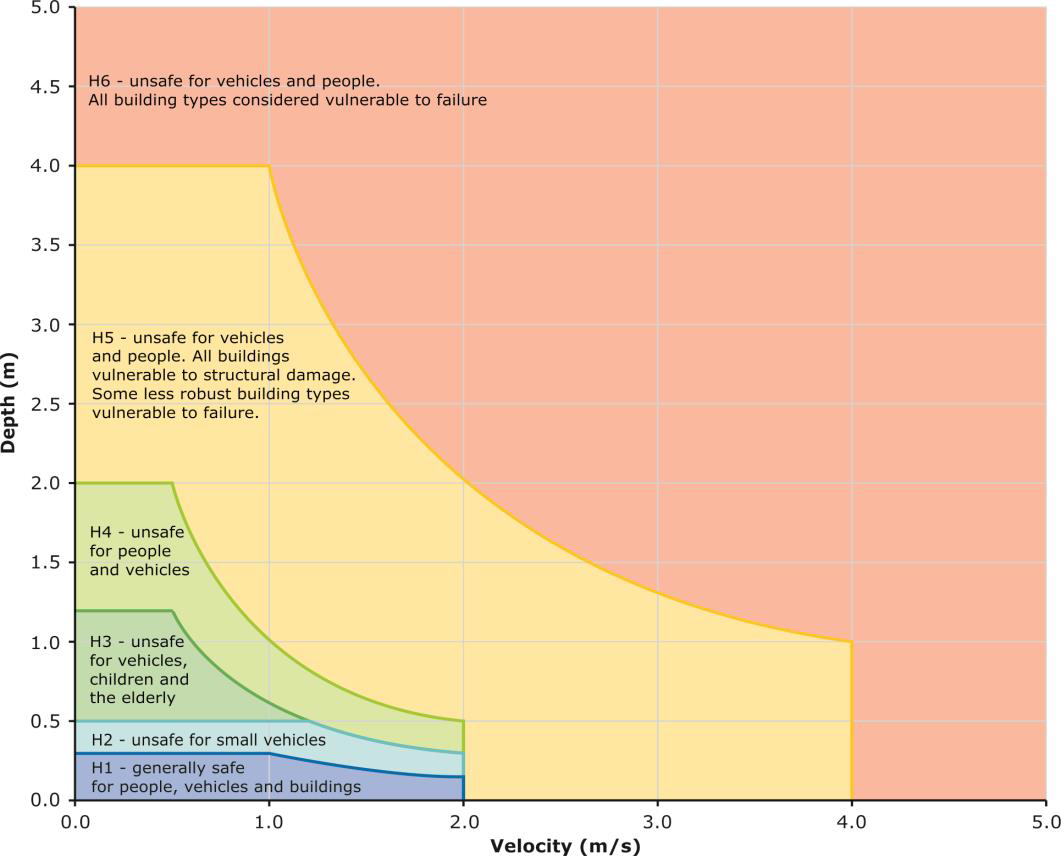
\includegraphics[width=0.7\textwidth]{images/results/original_hazard.png}
\caption{Original 6-level flood hazard vulnerability curves and thresholds, highlighting the $H_5$ boundary, adapted from \cite{Smith2016}.}
\label{fig:original_hazard}
\end{figure}

% Define the 15-level color palette from the simulator (6-digit HTML hex)
\definecolor{flevelOne}{HTML}{FFF176}
\definecolor{flevelTwo}{HTML}{FFD54F}
\definecolor{flevelThree}{HTML}{FFB74D}
\definecolor{flevelFour}{HTML}{FFA726}
\definecolor{flevelFive}{HTML}{FF8A65}
\definecolor{flevelSix}{HTML}{FF7043}
\definecolor{flevelSeven}{HTML}{F4511E}
\definecolor{flevelEight}{HTML}{E64A19}
\definecolor{flevelNine}{HTML}{D84315}
\definecolor{flevelTen}{HTML}{E53935}
\definecolor{flevelEleven}{HTML}{C62828}
\definecolor{flevelTwelve}{HTML}{B71C1C}
\definecolor{flevelThirteen}{HTML}{880E4F}
\definecolor{flevelFourteen}{HTML}{4A148C}
\definecolor{flevelFifteen}{HTML}{1A001A}

\begin{table}[h!]
\centering
\caption{Water depth intervals and color visualization matrix.}
\label{tab:hydraulic_scale}
\small
\begin{tabular}{|c|c|c|c|l|}
\hline
\textbf{Level} & \textbf{Water Depth Range (m)} & \textbf{\em Visual Sample} & \textbf{Hex Code} & \textbf{Severity Description} \\ \hline
1  & $0.20 \le h < 0.40$  & \cellcolor{flevelOne}       & \#FFF176 & H1 - Minor Pedestrian Hazard \\ \hline
2  & $0.40 \le h < 0.60$  & \cellcolor{flevelTwo}       & \#FFD54F & H2 - Small Vehicle Instability \\ \hline
3  & $0.60 \le h < 0.80$  & \cellcolor{flevelThree}     & \#FFB74D & H3 - Widespread Vehicle Instability \\ \hline
4  & $0.80 \le h < 1.00$  & \cellcolor{flevelFour}      & \#FFA726 & H4 - Severe Danger to People \\ \hline
5  & $1.00 \le h < 1.20$  & \cellcolor{flevelFive}      & \#FF8A65 & H5 - Major Internal Content Damage \\ \hline
6  & $1.20 \le h < 1.40$  & \cellcolor{flevelSix}       & \#FF7043 & H6 - High Wading and Rescue Hazard \\ \hline
7  & $1.40 \le h < 1.60$  & \cellcolor{flevelSeven}     & \#F4511E & H7 - Hydrostatic Pressure Accumulation \\ \hline
8  & $1.60 \le h < 1.80$  & \cellcolor{flevelEight}     & \#E64A19 & H8 - Non-Structural Component Failure \\ \hline
9  & $1.80 \le h < 2.00$  & \cellcolor{flevelNine}      & \#D84315 & H9 - Structural Damage Threshold \\ \hline
10 & $2.00 \le h < 2.50$  & \cellcolor{flevelTen}       & \#E53935 & H10 - First-Floor Submersion Risk \\ \hline
11 & $2.50 \le h < 3.50$  & \cellcolor{flevelEleven}    & \#C62828 & H11 - Complete First-Floor Submersion \\ \hline
12 & $3.50 \le h < 5.00$  & \cellcolor{flevelTwelve}    & \#B71C1C & H12 - Structural Integrity Failure Risk \\ \hline
13 & $5.00 \le h < 8.00$  & \cellcolor{flevelThirteen}  & \#880E4F & H13 - Multi-Story Inundation \\ \hline
14 & $8.00 \le h < 12.00$ & \cellcolor{flevelFourteen}  & \#4A148C & H14 - Extreme Infrastructure Failure \\ \hline
15 & $h \ge 12.00$        & \cellcolor{flevelFifteen}\color{white} & \#1A001A & H15 - Maximum Structural Collapse Limit \\ \hline
\end{tabular}
\end{table}


\section{Discussion of Modeling and Computational Limitations}

Acknowledging the operational boundaries of this research is essential for correctly interpreting the simulation results. 
The main limitations encountered during this study are detailed below:

\begin{itemize}
    \item \textbf{Computational Constraints and Grid Resolution}: Simulating a 14-hour catastrophic event over a 
    high-resolution $5\text{ m} \times 5\text{ m}$ grid introduces a massive computational burden. Due to hardware 
    limitations and prohibitive processing times per simulation run, a single-scenario approach was mandatory. 
    Consequently, iterative calibration and multi-scenario runs were outside the feasible scope of this thesis.
    \item \textbf{Stationary Roughness Parameters}: A uniform Manning’s coefficient ($n$) was assigned to urban and 
    rural zones based on standard literature. In reality, land cover resistance changed dynamically during the flood; 
    however, due to the aforementioned time constraints, a sensitivity analysis on roughness variations could not be 
    performed.
    \item \textbf{Fixed-Bed Assumption vs. Solid Transport}: The simulator operates under a fixed-bed hydraulic assumption. 
    The real-world event of October 29 was characterized by massive geomorphic changes, including severe sediment erosion, 
    uprooted vegetation, and thousands of swept vehicles blocking bridges. The exclusion of this floating debris transport 
    explains minor localized discrepancies where the model might underestimate water levels upstream of clogged bridges.
\end{itemize}


\section{Temporal Evolution of the Flood Simulation}

This section presents the spatio-temporal progression of the simulated flood event across the study area during the 14-hour 
simulated window. Due to the high spatial resolution of the computational grid ($5\text{ m} \times 5\text{ m}$ cells), specific 
key milestones were selected to illustrate the dynamics of the water flow rather than displaying continuous hourly outputs.

\begin{figure}[htbp]
    \centering
    % Panel A: t = 3h
    \subfigure[$t = 3\text{h}$]{
        \label{fig:depth_3h}
        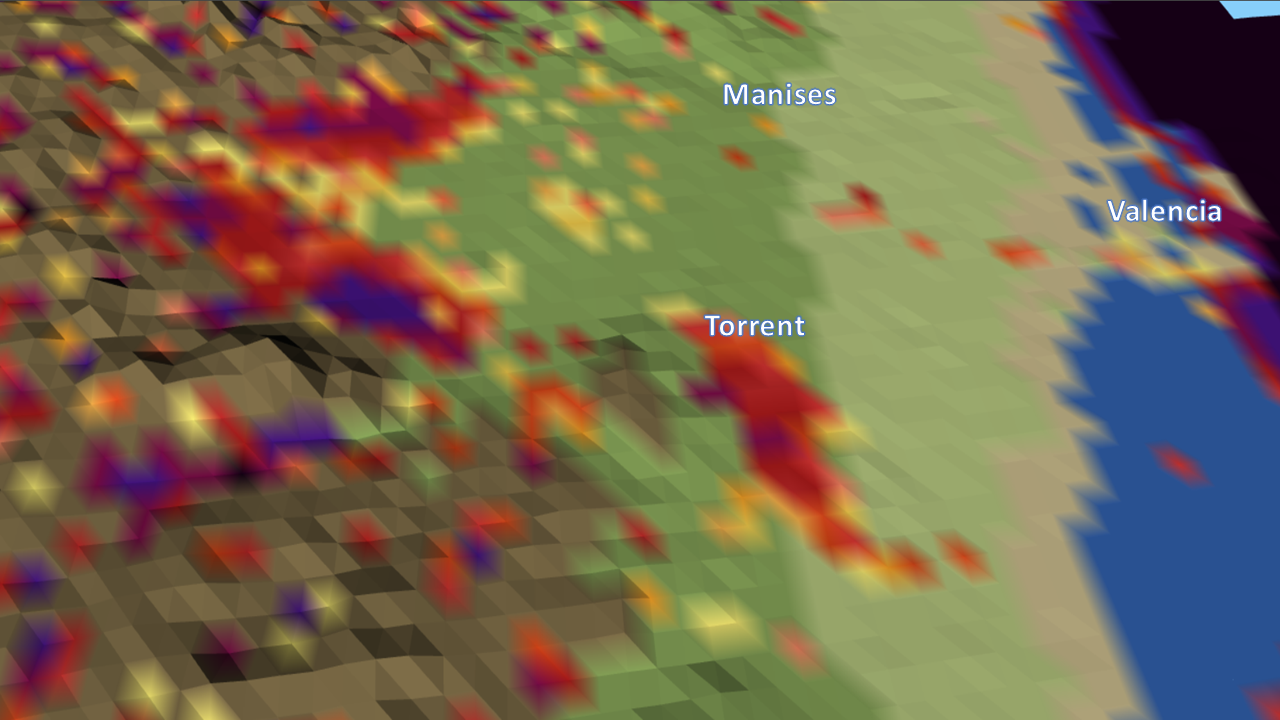
\includegraphics[width=0.7\textwidth]{images/results/water_depth_3h.png}
    } \\ % <- Este salto de línea fuerza la disposición vertical

    % Panel B: t = 7h
    \subfigure[$t = 7\text{h}$]{
        \label{fig:depth_7h}
        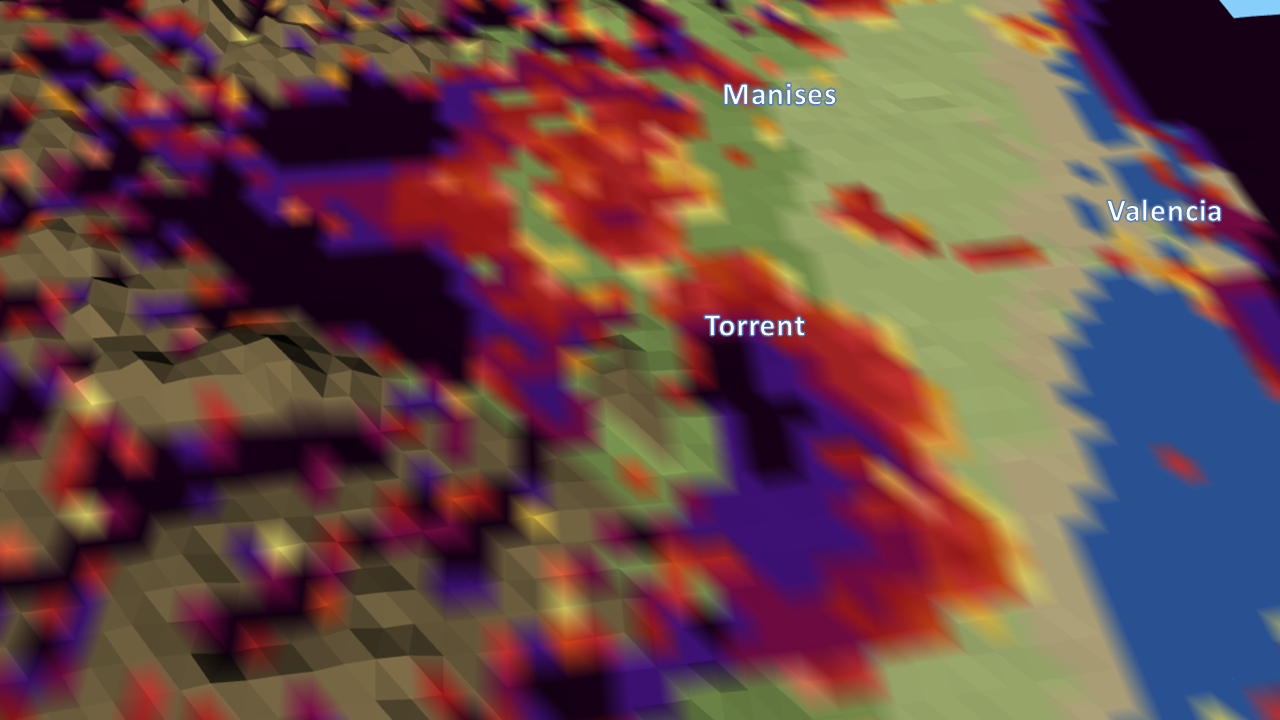
\includegraphics[width=0.7\textwidth]{images/results/water_depth_7h.png}
    } \\ % <- Otro salto de línea

    % Panel C: t = 14h
    \subfigure[$t = 14\text{h}$]{
        \label{fig:depth_14h}
        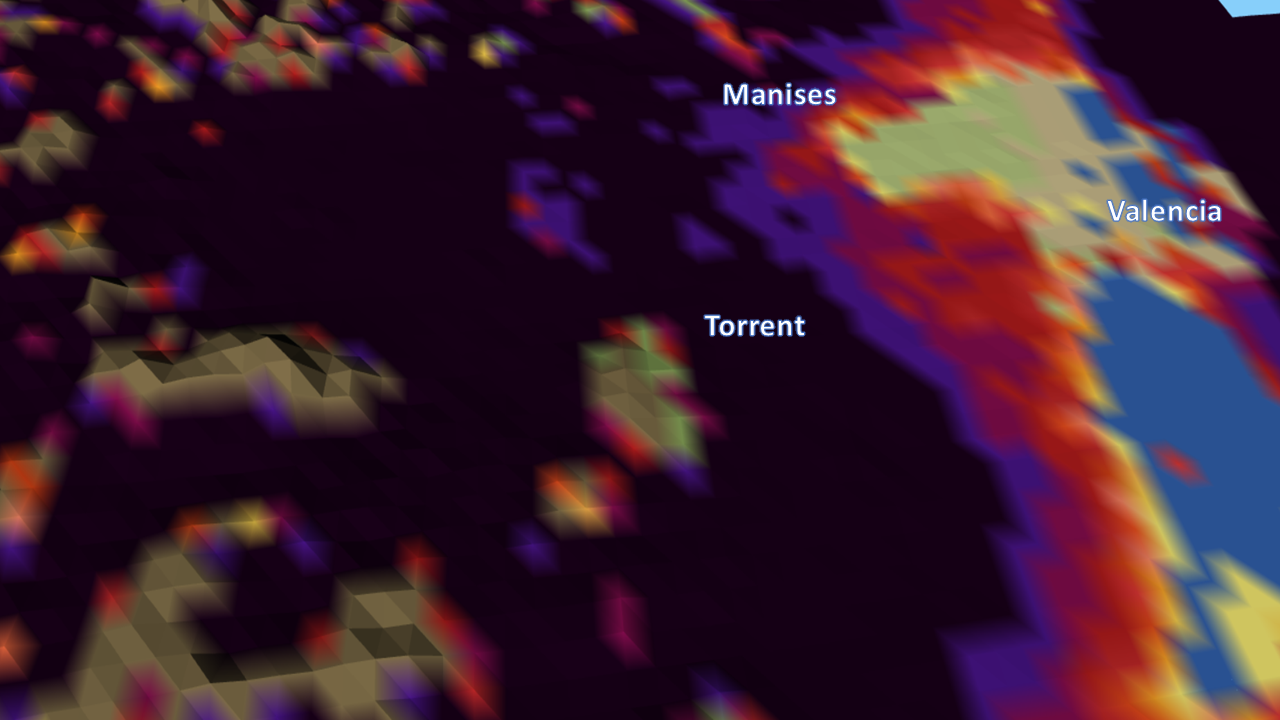
\includegraphics[width=0.7\textwidth]{images/results/water_depth_14h.png}
    }
    
    \caption{Multi-panel map showing the simulated water depth ($h$) progression at $t = 3\text{h}$, $t = 7\text{h}$, and $t = 14\text{h}$ using a standardized color scale.}
    \label{fig:water_depth_progression}
\end{figure}


\section{Visual Validation via Strategic Control Points}

\subsection{Control Point 1: Paiporta}

This section evaluates the visual correlation at Control Point 1 (Paiporta) by comparing the numerical simulation outputs 
against the empirical satellite references. The hydraulic state at $T+10$ hours—representing 20:00 CET, given that the 
historical flood onset is estimated around 07:00 AM—is contrasted directly with the reference map shown in \ref{fig:estimated_flood_paiporta}.

\begin{figure}[htbp]
    \centering
    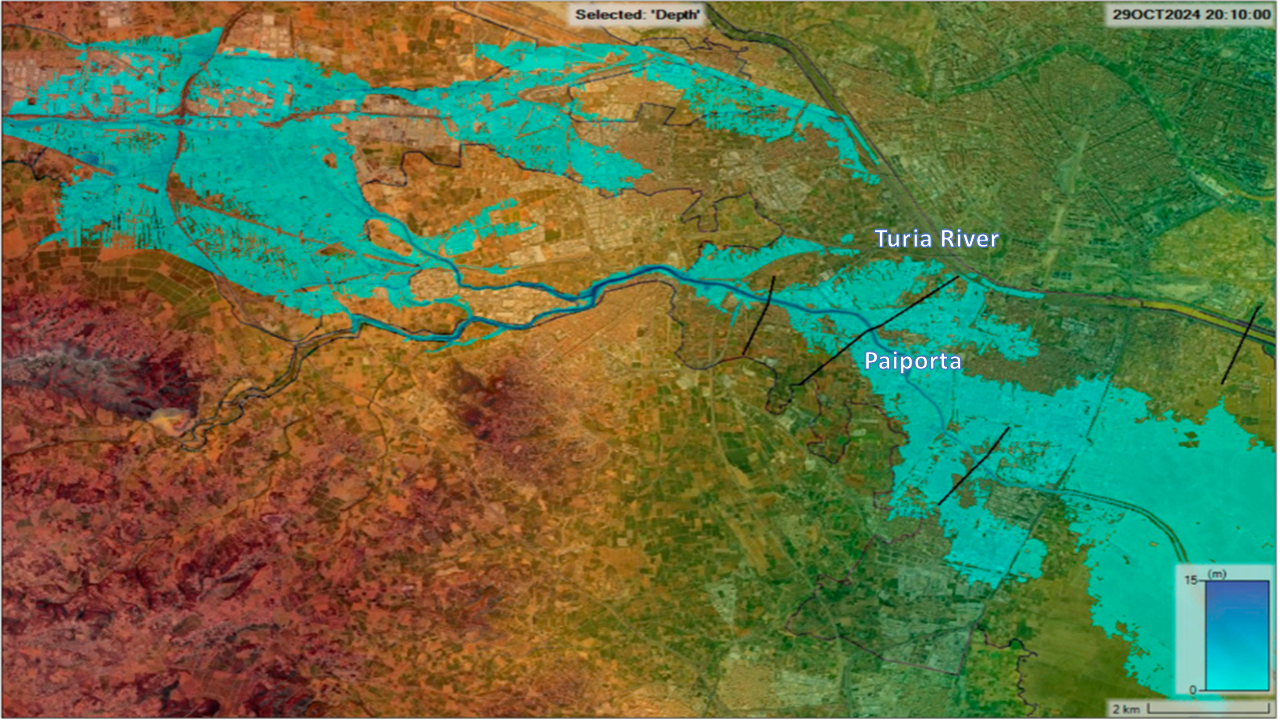
\includegraphics[width=0.9\textwidth]{images/results/estimated_flood_paiporta.png}
    \caption{Estimated flood extent at Control Point 1 (Paiporta) based on empirical satellite data.}
    \label{fig:estimated_flood_paiporta}
\end{figure}

As observed when comparing the empirical footprint with the simulated close-up grid in \ref{fig:sim_paiporta_1} and the wider 
domain perspective in \ref{fig:sim_paiporta_2}, the numerical model generates a higher volume of accumulated water distributed 
over a significantly larger surface area. Notably, the simulated flow even overwashes the artificial and natural topographic 
barriers formed by the main riverbeds, including the new Turia River diversion channel.

\begin{figure}[htbp]
    \centering
    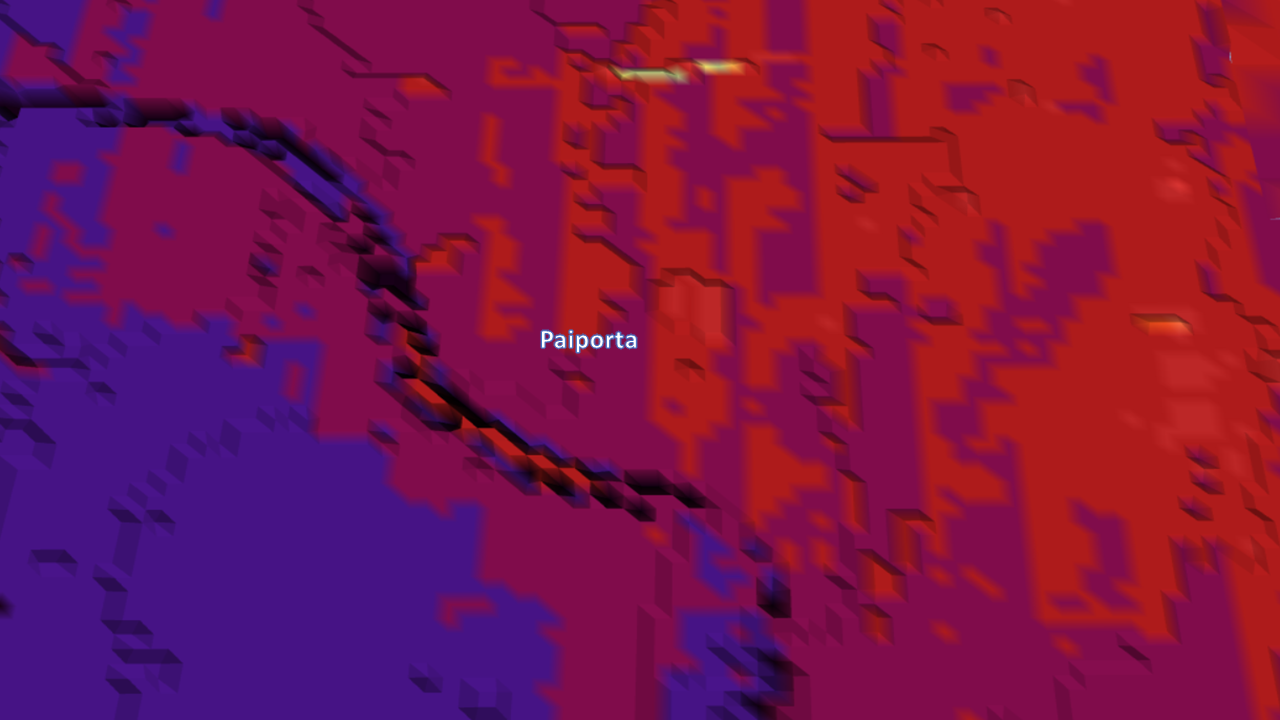
\includegraphics[width=0.9\textwidth]{images/results/sim_paiporta_1.png}
    \caption{}
    \label{fig:sim_paiporta_1}
\end{figure}

\begin{figure}[htbp]
    \centering
    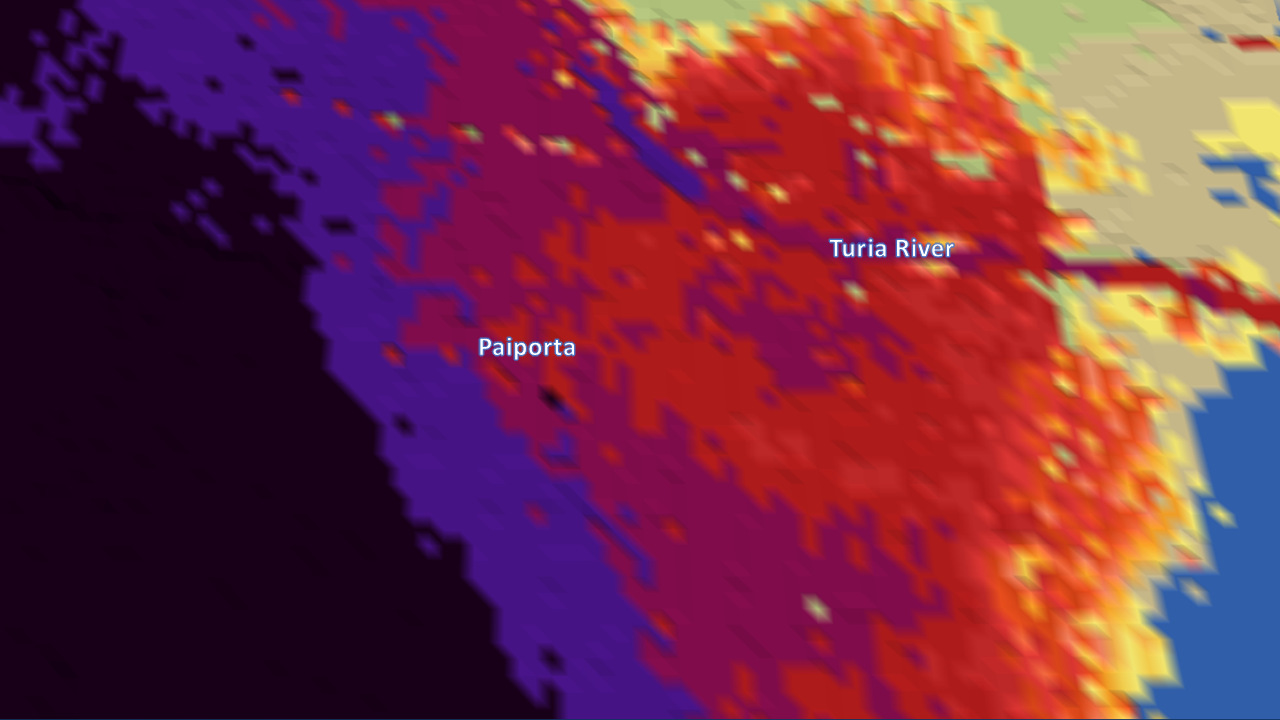
\includegraphics[width=0.9\textwidth]{images/results/sim_paiporta_2.png}
    \caption{}
    \label{fig:sim_paiporta_2}
\end{figure}

This localized water ponding and spatial overestimation can be scientifically attributed to two primary modeling factors:

\begin{itemize}
    \item \textbf{Underestimated Flow Velocity}: A lower numerical velocity within the computational grid slows down the 
    downstream propagation of the flood wave. This deceleration causes an artificial backup, increasing the water depth 
    ($h$) and retention times within the upstream urban nodes.
    \item \textbf{Fixed-Bed Simulation Constraints}: Because the simulator operates under a static terrain assumption, it 
    lacks the capacity to model dynamic geomorphic modifications, sediment transport, or macro-debris accumulation. In the 
    real-world event of October 29, thousands of swept vehicles and uprooted vegetation created physical blockages and 
    macro-tamonaments in narrow street canyons and bridges. Lacking these physical barriers, the simulated water expands 
    freely into urban sectors that were topographically or physically shielded by debris in reality.
\end{itemize}

Furthermore, the significant water accumulation visible in the downstream areas of the simulation grid—specifically near 
the Albufera lagoon and the Mediterranean coastline in \ref{fig:sim_paiporta_2}—further supports the hypothesis of an underestimated 
flow velocity. This velocity deficit alters the overall drainage dynamics across the low-lying alluvial plains, forcing the
simulated excess water volume to pool extensively as it approaches the coastal boundary condition rather than discharging 
dynamically into the sea.


\subsection{Control Point 2: Industrial Corridor and Agricultural Flanks (A-3 Axis)}

This control point analyzes the hydrodynamic behavior of the flood wave as it traverses a highly heterogeneous landscape 
along the A-3 highway corridor. As shown in the satellite overview map \ref{fig:poligono_overview}, this industrial park 
was historically developed over reclaimed agricultural land. Topographically, the zone is confined within a natural valley 
between two prominent elevated terrains. Strategically, this corridor serves as the primary hydraulic conduit connecting the 
\textit{Circuit Ricardo Tormo} (upstream, which suffered catastrophic structural destruction during the real event) and the 
\textit{Centro Comercial Bonaire} (downstream, one of the most severely impacted commercial zones).

\begin{figure}[htbp]
    \centering
    \includegraphics[width=0.9\textwidth]{images/results/poligono_overview.png}
    \caption{}
    \label{fig:poligono_overview}
\end{figure}

The core objective of this control point is to evaluate how effectively the simulator replicates land-use-driven velocity 
variations by applying distinct surface roughness values (Manning's $n$ coefficients) to different terrain categories. The 
spatio-temporal progression of this phenomenon is documented across three sequential snapshots in \ref{fig:poligono_progression}, 
which captures the flood wave's morphological transformation.

\begin{figure}[htbp]
    \centering
    % Panel A: t = 3h
    \subfigure[$t = 2.5\text{h}$]{
        \label{fig:sim_poligono_1}
        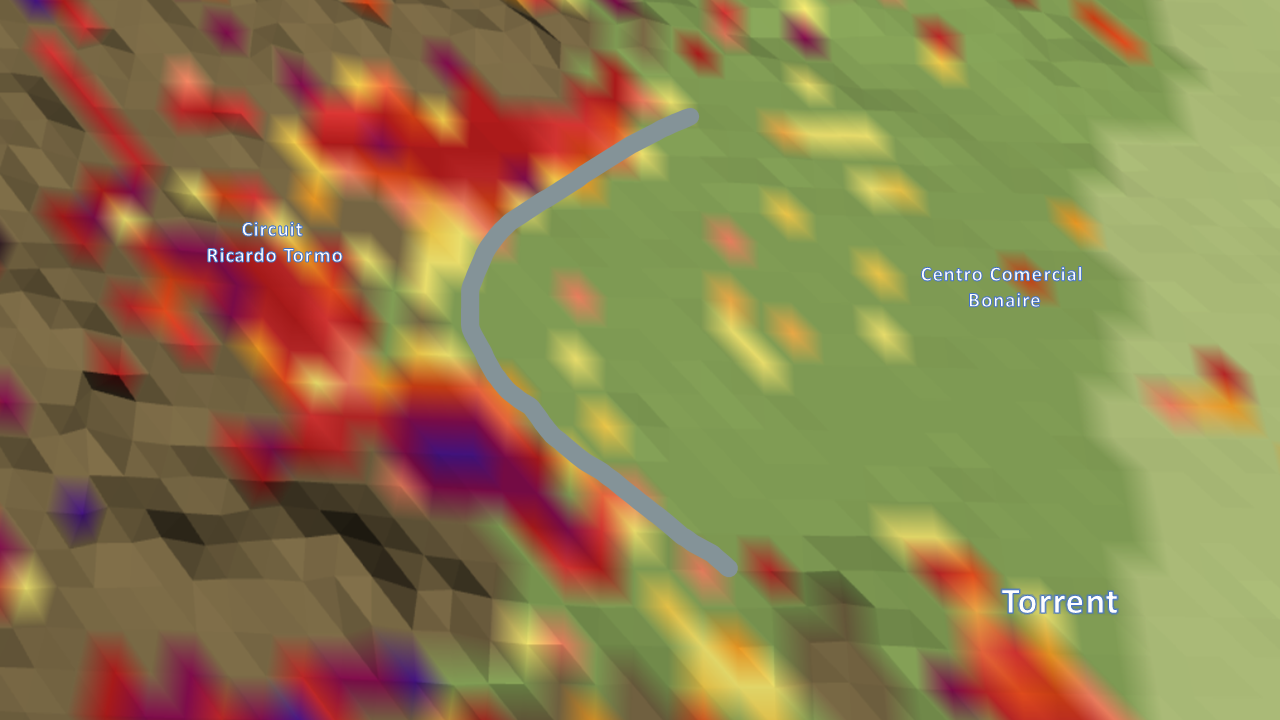
\includegraphics[width=0.7\textwidth]{images/results/sim_poligono_1.png}
    } \\ % <- Este salto de línea fuerza la disposición vertical

    % Panel B: t = 7h
    \subfigure[$t = 4.25\text{h}$]{
        \label{fig:sim_poligono_2}
        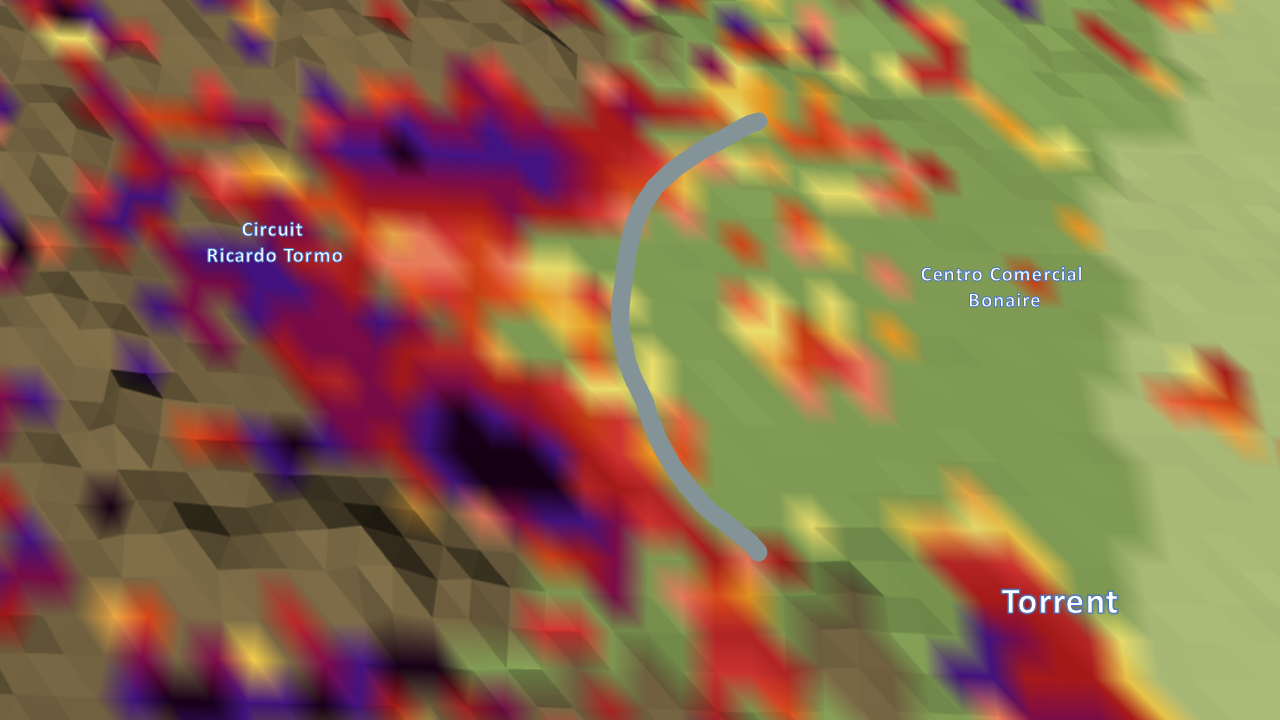
\includegraphics[width=0.7\textwidth]{images/results/sim_poligono_2.png}
    } \\ % <- Otro salto de línea

    % Panel C: t = 14h
    \subfigure[$t = 7\text{h}$]{
        \label{fig:sim_poligono_3}
        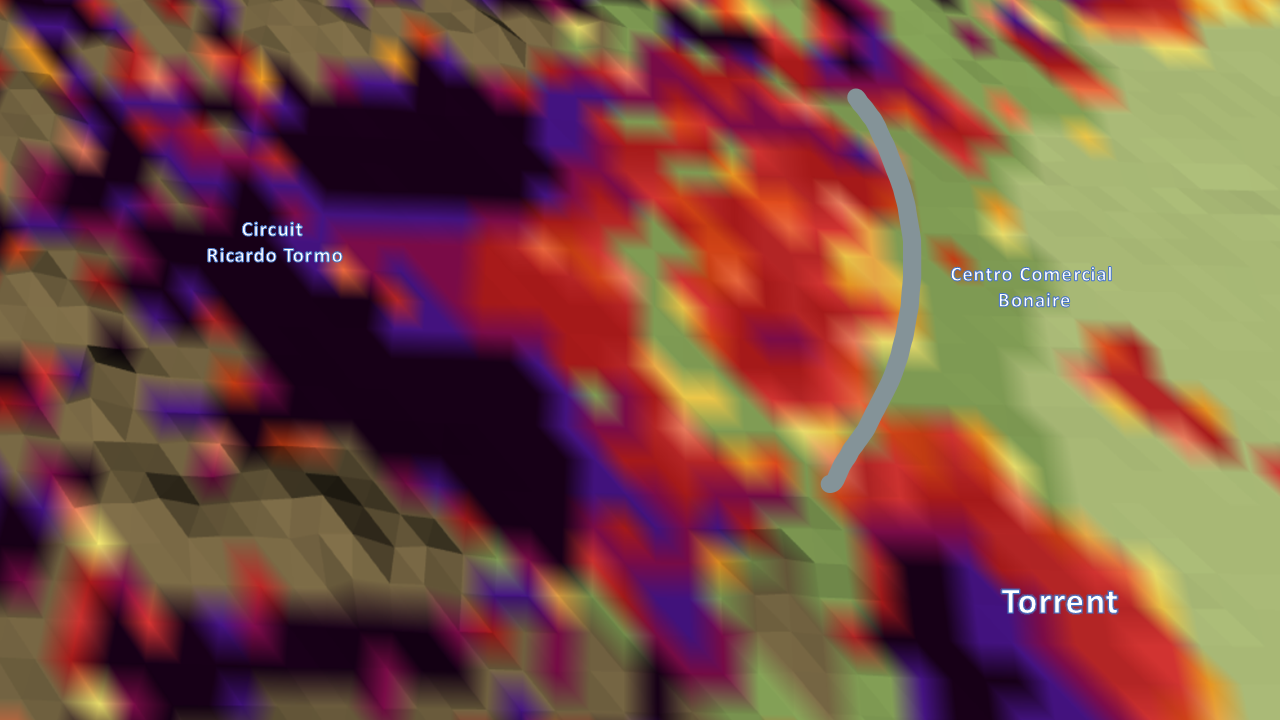
\includegraphics[width=0.7\textwidth]{images/results/sim_poligono_3.png}
    }
    
    \caption{Multi-panel map showing the simulated water depth ($h$) progression at $t = 3\text{h}$, $t = 7\text{h}$, and $t = 14\text{h}$ using a standardized color scale.}
    \label{fig:poligono_progression}
\end{figure}

The simulation yields several critical hydrodynamic insights that validate the model's physics:

\begin{itemize}
    \item \textbf{Agricultural Energy Dissipation and Pooling:} In the early stages of the propagation ($T+2.5\text{h}$ and 
    $T+4.25\text{h}$), large volumes of water accumulate rapidly within the agricultural fields flanking both sides of the 
    industrial park. Due to the high Manning's roughness coefficient assigned to croplands, the flow velocity decreases 
    significantly. According to the principle of mass conservation, this deceleration induces a severe hydraulic backup, 
    resulting in elevated water depths represented by the critical red and purple bands in \ref{fig:sim_poligono_1} and 
    \ref{fig:sim_poligono_2}.
    
    \item \textbf{Industrial Grid Acceleration:} Conversely, as the water penetrates the boundaries of the industrial park, it 
    encounters a completely different surface texture. The lower Manning's $n$ values associated with paved roads, asphalt 
    logistics yards, and concrete surfaces offer minimal friction to the sheet flow. Consequently, the water experiences rapid 
    acceleration upon entry. 
    
    \item \textbf{Wave Front Morphological Inversion:} This localized velocity differential induces a stark geometric transformation 
    in the flood wave front, shifting from a \textit{convex} shape into a distinctly \textit{concave} profile along the advancement 
    axis. As visualized across the time steps, the high-velocity "tongue" of the flood shoots forward through the smooth industrial 
    grid, while the lateral wings of the wave remain lagged behind within the high-friction agricultural fields.
    
    \item \textbf{Depth vs. Velocity Trade-off:} Because the water is channeled and accelerated within the industrial park, the 
    steady-state water depths inside the polygon remain visibly lower than those reached in the adjacent rural fields. However, 
    this velocity surge carries a higher destructive potential downstream. The simulation demonstrates that the industrial 
    infrastructure effectively acted as a high-speed hydraulic highway, accelerating the arrival time of the flood wave toward 
    highly populated and vulnerable downstream receptors, precisely replicating the historical flash-flood trajectory that 
    devastated the \textit{Centro Comercial Bonaire} area.
\end{itemize}

In conclusion, the visual sequence successfully demonstrates that the simulator does not merely treat the terrain as a uniform 
plane. By producing this intricate concave-convex wave distortion, the model proves highly sensitive to land-use variations, 
validating its capability to simulate the real-world micro-hydraulics of the October 29 catastrophe.
